\chapter{Refraction and Lenses}

Over the next few classes, we're going to examine how telescopes work,
but first we need to figure out some aspects of the behavior of light
when it passes through transparent materials such as glass.

The apparatus for this lab consists of a light source that produces a set
of parallel beams from lasers, along with a variety of transparent and
reflective objects for the light to interact with.  All of these objects
can be attached magnetically to a small whiteboard, so that they can be
easily positioned in various ways.

\paragraph{Part 1: Refraction.}
Plug in the light source and attach it to the whiteboard.  Put
the clear plastic rectangle in front of the source, so that
the light rays hit it at an angle like this:

%\centerline{\epsfxsize 3in\epsfbox{figs/lensfig1.eps}}
\centerline{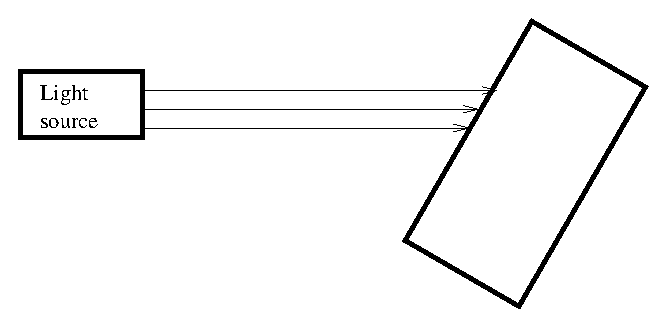
\includegraphics[width=3in]{figs/lensfig1.eps}}


Put a piece of paper under the rectangle.  Trace the outline of the rectangle
on the paper.  Also, trace the path of one of the rays as it enters
the rectangle, and the same ray as it exits the other side.  Use
a straightedge to make sure your lines are straight.
Then remove the paper, and draw a straight line connecting the points
where the ray entered and exited the rectangle. 
You should end up
with a picture like this:

\centerline{\epsfxsize 3in\epsfbox{figs/lensfig2.eps}}



The light ray bends when it enters the plastic.  This phenomenon is
called {\it refraction}.  There is a rule called Snell's Law that
describes the amount of bending:
$$
\sin\theta_i=n\sin\theta_r.
$$
In this law, $n$ is a constant called the {\it index of refraction} of 
the material.  The angles $\theta_i$ and $\theta_r$ are called the
angle of incidence and angle of refraction.  They're defined to be the
angles the light ray makes with a line perpendicular to the surface
where the light ray entered the material, as shown here:

\centerline{\epsfxsize 3in\epsfbox{figs/lensfig3.eps}}


It's easier to measure the angles that the light ray makes with
the \textit{edge} of the rectangle, instead of the angle that it makes with
the \textit{perpendicular line}.  So measure the two angles
indicated by the arrows in the picture, and use them
to determine the angles $\theta_i$ and $\theta_r$.


\vskip 1.5in

Now use these angles in Snell's Law (the equation above) to determine
the value of the index of refraction $n$.

\vskip 1.5in

The value of $n$ is supposed to be the same no matter what incident angle
you choose.  To test this, rotate the rectangle so that the light
rays hit it at a different angle.  Repeat the procedure above to determine
$\theta_i,\theta_r$, and $n$.  Do you get roughly the same value of $n$ as
before?

\vskip 3in

\paragraph{Part 2: Total internal reflection.}
Once the light ray has entered the surface, it has to bend again
in order to get back out.  (That's why the rays that leave the rectangle
end up parallel to the ones that go in.)  Sometimes the rays can't bend
enough to make it back out, and in this case they are reflected, bouncing
back and forth inside the material.  To see this, take the long, thin
rectangular piece of plastic, and arrange it so that one of the light
rays enters at a slight angle like this:

\centerline{\epsfxsize 3in\epsfbox{figs/lensfig4.eps}}



If you adjust the angles right, you should be able to see the light ray
bounce back and forth from side to side inside the plastic.  
Using total internal reflection, 
light signals can be transmitted over very great distances through
fiber optic cables.

\paragraph{Part 3: Lenses.}
A curved piece of refracting material can act as a lens, bringing
light to a sharp focus.  Lenses are found in your eyes, as well as
corrective lenses (eyeglasses or contact lenses), cameras,
microscopes, etc.  For this course, of course, the most important
application of lenses is in telescopes.  We'll examine how telescopes
work in future classes.  For the moment, let's just figure
out some general properties of lenses.

Take one of the three lenses labeled 1,2,3, and place it in front
of the light source.  You should see the light rays bending to
come (approximately) to a {\it focal point} on the far side of the lens.  
The {\it focal length} of a lens is defined to be the distance from the center
of the lens to the focal point.  Determine the focal lengths of all
three lenses.  (The easiest way to do this is to mark the focal point
on the white board, and also to mark the edges of the lens.  Then
you can remove the lens and measure the distance from the focal
point to the middle of the lens.)

\vskip 2.5in

These three lenses are all called {\it converging} lenses, because
they cause the light to converge to a point.  There are also {\it diverging}
lenses, which generally have concave rather than convex surfaces.  Put
the lens labeled 5, which is a diverging lens, 
in front of the light source and see what it does.
A diverging lens causes the light rays to spread out {\it as if} all the
rays were coming from a focal point on the same side of the lens
as the light source.

To see how this works, trace the paths of several of the rays 
after they exit the lens.  Also, mark the positions of the edges
of the lens.  Now remove the lens and, using a straightedge, extend
the rays {\it backwards} until they come together at a single point.  
The distance from the center of the lens to this focal point is
called the focal length of the lens.  Measure the focal length
of this diverging lens.

\vskip 1in

\paragraph{Part 4: Combinations of lenses.}
Put one of the converging lenses (1,2,3) in front of the light source, and
then put another one of the converging lenses right in front of the first
one.  The two lenses should behave approximately like a single lens.
Is it a converging or a diverging lens?  How does the focal length of
the combined lenses compare with the focal length of the original
lenses?  (I'm not looking for a measurement here, just a general
observation.)

\vskip 1.5in

Try the same thing with a combination of a converging and a diverging
lens.  Does the combination behave like a converging lens or a diverging
lens?  

\vskip 1.5in

Remove the other lenses and place the lens labeled 4 in front
of the light source.  Is this a converging lens or a diverging lens?
Is its focal length larger or smaller than those of lenses 1,2,3,5?

\vskip 1.5in

Place the diverging lens (5) right in front of lens 4.  Does the combination
of lenses 4 and 5 behave like a converging lens or a diverging lens?

\vskip 1.5in

By now, you should have seen that sometimes a combination of a converging
and a diverging lens acts like a converging lens, and sometimes it
acts like a diverging lens.  There is a general rule for predicting,
for any given pair of lenses, which way the combination of the two
will behave.  Can you guess what this general rule might be?


